\chapter{Time Projection Chamber}
\label{sec:tpc}
	\textcolor{red}{Using (2010 -- a little old) https://cds.cern.ch/record/1302071/files/CERN-PH-EP-2010-047.pdf}
	
	A~\acf{TPC} is a~type of gaseous detector that uses the~drift in an~electric field of free charges (electrons and cations, \textcolor{red}{also anions if attachment is considered}) produced by an~ionizing particle to reconstruct its 3D~trajectory. When placed inside a~magnetic field, the~momentum of the~incident particle can be inferred from the~curvature of its trajectory. Particle identification is also possible using the~ionization energy loss inside the~\ac{TPC}.
	
	The original \ac{TPC} used in the~PEP-4 experiment at SLAC (Figure~\ref{fig:pep4}) was a $2\times2$~m cylinder with a~central cathode that produced a~strong electric field, making the~ionization electrons drift towards one of the bases. The~readout consisted of \ac{MWPC}s, where electrons are accelerated towards the~anode wires enough to further ionize the~gas and cause an avalanche.
	
	\begin{figure}
		\centering
		\includegraphics[width=0.7\textwidth]{pep4_tpc.png}
		\caption{Schematic view of the~PEP-4 \ac{TPC}~\cite{pep4}.}
		\label{fig:pep4}
	\end{figure}
	
	When a~charged particle crosses the~volume of a~\ac{TPC}, it loses energy by excitation and ionization of the detector gas (\textcolor{red}{how much -- from dE/dx + density $\rightarrow$ footnote?}). Most ionizing collision produce a~single ionization electron, sometimes a~few secondary electrons are produced close to the~collision vertex. In rare cases, the~ionization electron has energy large enough to create a measurable track, such an~electron is called a~$\delta$\nobreakdash-electron (\textcolor{orange}{terminology, just like bellow -- technically it's a (primary) ionization electron causing other (secondary) ionization}). \textcolor{red}{Penning transfer (collisions, light -- factor 10 for gas gain in Ar/CO2 viz PDG CERN)?}
	
	\textcolor{red}{CERES/NA45 -- very inhomogeneous magnetic field}
	
	\section{Charge transport in gases}
		\subsection{Drift}
			Produced ionization electrons (\textcolor{orange}{terminology -- called ionization electrons in the rest of the thesis}) are accelerated towards the~readout by the~electric field inside the~chamber. At the same time, they lose speed by colliding with the~gas particles, quickly reaching a~constant (for a~given field $\mathbf{E}, \mathbf{B}$) mean drift velocity. The~electrons might be absorbed by electronegative impurities, such as halides and oxygen.
			
			In many gases (called "hot", e.g., Ar or CH$_4$), the~drift velocity is much greater than that of their thermal motion thanks to a~high proportion of elastic collisions. On the other hand, "cold" gases like CO$_2$ have a higher proportion of inelastic collisions (e.g., thanks to the~excitation of rotational and vibrational states) and therefore much lower (\textcolor{orange}{value? magnitude (implied)?}) drift velocity. (\textcolor{orange}{def?})
			
			The ions produced by the~ionization lose a significant portion of their energy during each collision since their mass is close to the~mass of the~gas particles (\textcolor{orange}{see the source material -- average energy loss during collision $\Delta E = \frac{2m_i M}{(m_i+M)^2}$}, this way it's more accurate). This, together with their large collision cross section, makes their drift velocity much smaller and their energy is close to thermal. Since their momenta aren't randomized to such an~extent during collisions, their diffusion is smaller (\textcolor{orange}{more in the~sense of distribution of positions, could move this to the diffusion subsection}).
			
			The drift is also influenced by the~magnetic field. Langevin derived a~good approximation for the~drift velocity vector:
				\begin{equation}
					\label{eq:drift}
					\mathbf{v}_\text{d} = \left(\frac{\mathbf{E}}{\norm{\mathbf{E}}} + \omega\tau\frac{\mathbf{E}\times\mathbf{B}}{\norm{\mathbf{E}}\norm{\mathbf{B}}} + \omega^2\tau^2\frac{\mathbf{E}\cdot\mathbf{B}}{\norm{\mathbf{E}}\norm{\mathbf{B}}}\cdot \frac{\mathbf{B}}{\norm{\mathbf{B}}}\right) \frac{q\tau}{m(1+\omega^2\tau^2)}\norm{\mathbf{E}},
				\end{equation}
			where $q$ is the~charge of the particle, $m$ is its mass, $\tau$ is the mean time between collisions and $\omega = \frac{q}{m}\norm{\mathbf{B}}$ is the~Larmor frequency. In a~standard \ac{TPC}, $\mathbf{E}$ is nearly parallel to $\mathbf{B}$ and the~influence of the~magnetic field on the~drift is minimal. The~drift of ions is only negligibly influenced by the~magnetic field ($\omega\tau\sim10^{-4}$ is small due to the~low drift velocity \textcolor{orange}{-- better because it takes $\tau$ into account and differs only by E/B ratio}). \textcolor{red}{Lorentz angle for orthogonal fields $\tan\psi = -\omega\tau$ (deviation from electric field) -- maybe mention in the OFTPC section.} Without magnetic field, we can write
				\begin{equation}
					\mathbf{v}_d = \frac{q\tau}{m} \mathbf{E} = \mu \mathbf{E},
				\end{equation}
			where $\mu$ is called charge mobility.
			
		\subsection{Diffusion}
			Due to collisions a~cloud of electrons or ions originating from the~same point will show a~Gaussian density distribution at time $t$ while drifting in the~electric field $\mathbf{E} = (0,0,E_z)$:
				\begin{equation}
					\rho(x,y,z,t) = (4\pi Dt)^{-\frac{3}{2}} \exp\left(-\frac{x^2+y^2+(z-v_dt)^2}{4Dt}\right),
				\end{equation}
			where the diffusion coefficient $D$ can be expressed as
				\begin{equation}
					D = \frac{\lambda^2}{3\tau} = \frac{\lambda v_\text{d}}{3} = \frac{v_\text{d}^2\tau}{3} = \frac{2\varepsilon\tau}{3m},
				\end{equation}
			where $\lambda$ is the mean free path and $\varepsilon$ the mean energy. The lateral diffusion width $\sigma_x$ after a drift distance $L$ can be expressed as
				\begin{equation}
					\sigma_x^2 = 2Dt = \frac{4\varepsilon L}{3qE}.
				\end{equation}
			The minimal diffusion width is given by the~lowest possible energy of the~particles $\varepsilon_\text{th} = \frac{3}{2}kT$ (corresponding to thermal motion):
				\begin{equation}
					\sigma_{x, \,\text{min}}^2 = \frac{2kTL}{qE}.
				\end{equation}
			For electrons in "cold gases" (e.g., Ar/CO$_2$ mixture), the diffusion approaches this limit up to a~certain field intensity ($\sim 100~\text{V}/\text{cm}$ at 1~atm pressure)\footnote{\textcolor{red}{For us 0.45~mm, quite close to the actual diffusion 0.5-0.7~mm.}}. In reality, the~transversal diffusion of electrons can differ significantly from their longitudinal diffusion and simulations are necessary to get a~precise result.
			
			In most \ac{TPC}s, the~transversal (but not the~longitudinal) diffusion is reduced by the~magnetic field, since it is parallel to the~electric field and curves the~diffusing electrons around their mean trajectory:
				\begin{equation}
					\label{eq:difmag}
					\frac{D_\text{T}(B)}{D_\text{T}(0)} = \frac{1}{C+\omega^2\tau_2^2},
				\end{equation}
			where $C$ and $\tau_2$ are parameters dependent on the~gas used. At low intensity of the~magnetic field, we can use an~approximation $C\approx1$ and $\tau_2\approx\tau$.
	
	\section{Readout}
		\subsection{Multi-Wire Proportional Chamber}
			In most \textcolor{red}{(2010 -- almost all)} \ac{TPC}s operated in experiments \acf{MWPC} was used for the~readout. The electrons enter the chamber through a~cathode grid and get accelerated in the~strong electric field towards the~thin anode wires and create a~Townsend avalanche, multiplying the~signal. \textcolor{red}{Alternating with field wires?} The~trajectory can be reconstructed using pulses from each separate wire. Segmented cathode is also often used for the readout of produced cations. \textcolor{red}{Gating grid (reduction of space charge effect, blocking backflow of ions?, closed for electrons B=0, $\Delta V$, static mode (loss of 25\% el.) x opening on trigger)? (gas amplification $>10000$ required for good SNR, 100-200~ns shaping time), figure?}
			
		\subsection{Gas Electron Multiplier}
			The~\acf{GEM} is a~thin metal\nobreakdash-coated polymer sheet with a~high density of small holes. The amplification is achieved by applying voltage on the~metal layers, creating a strong electric field inside the~holes and causing avalanches. Double or triple stack of \ac{GEM}s is usually used to create a~sufficient gain. From the last foil, the~electrons drift to a~segmented anode where the~signal is read. The~backflow of cations is reduced compared to \ac{MWPC}. An~example simulation of an avalanche inside \ac{GEM} is shown in Figure~\ref{fig:gemsim}. \textcolor{red}{Parameters?}
			
			\begin{figure}
				\centering
				\includegraphics[width=0.8\textwidth]{gemsim.png}
				\caption{Garfield simulation of an avalanche in a \ac{GEM} hole~\cite{gemsim}.}
				\label{fig:gemsim}
			\end{figure}
		
		\subsection{Micromegas}
			In a~\ac{Micromegas} electrons pass through a~fine mesh (made out of very thin wires) into the~narrow amplification gap where they are multiplied in the~high field and read as signal on the~segmented anode. Very high field (30-80 kV/cm$^2$) is necessary to achieve sufficient gain. Cation backflow is heavily suppressed by the~mesh.
			
		\subsection{Parallel Plate Chamber}
			\textcolor{red}{..., microwell?}
			
			
	
	\section{Orthogonal Fields TPC at IEAP CTU}
	\label{sec:oftpc}
		At \ac{IEAPCTU}, we are going to use six identical atypical \ac{TPC}s with inhomogeneous toroidal magnetic field orthogonal to the~electric field, hereafter referred to as \acf{OFTPC}. It has the~shape of isosceles trapezoidal prism 16~centimeters high with triple\nobreakdash-\ac{GEM} readout on one of its bases. Dimensions of the~\ac{OFTPC} are discussed in detail in section~\ref{sec:coor} below. Throughout this thesis, we assume a~uniform electric field along the~$z$~axis with $E_z = -400$~V/cm. \textcolor{red}{Gas mixture used in the~detector (70/30) and its effect -- some graph with the mixture.}
		
		
		\subsection{Motivation and Associated Challenges}
			The~reasons for the~unusual field layout are mostly cost related:
				\begin{itemize}[nosep]
					\item we use permanent magnets instead of a~solenoid and parallel fields are difficult to accomplish this way,
					\item granularity of the~\ac{TPC} readout is limited in order to fit one SAMPA/SRS hybrid in each sector -- parallel fields would bend the~trajectories parallel to the~readout requiring more pads and different architecture.
				\end{itemize}
			In this thesis, we will show that such a~setup can reach a~similar energy resolution as common cylindrical \ac{TPC}s while reducing cost.
			
			The layout introduces two complications to the~track reconstruction -- the trajectory in inhomogeneous field is not circular and the drift is distorted by the magnetic field (see Equation~\ref{eq:drift}, in our case $\omega\tau \approx 0.08$ \textcolor{red}{for 0.3~T assuming $\mu\approx0.25$~T$^{-1}$, varies inside the detector}). The diffusion in such setup is larger since parallel orientation reduces diffusion by curling the~electrons in the $x$\nobreakdash-$y$ direction (see Equation~\ref{eq:difmag}) but for our relatively weak magnetic field and short drift distance the~difference is negligible.
	
		\subsection{Coordinate Systems and Dimensions}
		\label{sec:coor}
			In order to describe events in our detector, we use three distinct spaces: the~detector space $\mathcal{D}$, the~readout space $\mathcal{R}$ and the~pad space $\mathcal{P}$. Each space is later used to represent ionization electrons at different stages of the~detection process: their creation in the gas, their final position when hitting the readout plane, and finally their representation in the discrete pad space.
		
			\subsubsection{Detector Space}
				The~detector space $\mathcal{D}$ represents the~physical space of our detector. We describe it using Cartesian coordinates $(x,y,z)$. The~$z$-axis is the~detector's axis of symmetry, with its negative direction aligned with the~proton beam. The~origin $(0,0,0)$ is located at the~center of the~irradiated target. The~positive $x$\nobreakdash-axis passes through the~center of one the~\ac{OFTPC}s along the~intersection of its two planes of symmetry. The~$y$\nobreakdash-axis is then chosen to maintain a~right-handed coordinate system.
				
				Since the~detector has a~hexagonal symmetry, we use only one of its sectors in this work -- the~first sector $\mathcal{D}_1 \subset \mathcal{D}$ which is defined by the~condition:
					\begin{equation}
						(x,y,z) \in \mathcal{D}_1 \Leftrightarrow |y| \leq x\tan \frac{\pi}{6}.
					\end{equation}
				Simulations in this sector can be applied to all sectors by rotating the coordinates accordingly. The~volume of the~\ac{OFTPC} in this sector, which has the~shape of a~trapezoidal prism, has these boundaries:
					\begin{linenomath}
						\begin{align}
							x \in [x_\text{min},x_\text{max}] &= [6.51, 14.61] \;\text{cm},\\
							z \in [z_\text{min},z_\text{max}] &= [-8,8] \;\text{cm},\\
							y_\text{max}(x_\text{min}) = -y_\text{min}(x_\text{min}) &=  2.75\;\text{cm},\\
							y_\text{max}(x_\text{max}) = -y_\text{min}(x_\text{max}) &=  7.45\;\text{cm},
						\end{align}
					\end{linenomath}
				where $y_\text{max}(x)$ is the~maximal value of the~$y$-coordinate for a~given $x$. The~readout is located at $z = 8$~cm; for some purposes, we also define the distance to the~readout $d_r = 8\;\text{cm}-z$ as an~alternative to the~$z$-coordinate. \textcolor{red}{Keeping this paragraph as it is because the~\ac{OFTPC} volume is distinct from the~first sector and some parts of this thesis use the~space beyond this volume.}
				
				We also use spherical coordinates $(r,\theta,\varphi)$ with $\theta$ measured relative to the~$xy$ plane.
				
				\begin{figure}
					\centering
					\includegraphics[width=0.8\textwidth]{tpc_ggb.png}
					\caption{Schematics of the~first sector \ac{OFTPC} with detector space coordinates.}
					\label{fig:oftpc}
				\end{figure}
			
			\subsubsection{Readout Space}
				The~readout space $\mathcal{R}$ represents the~drift time and final positions of ionization electrons as measured by an~ideal continuous readout. We describe it using coordinates $(x',y',t)$, where $x'$ and $y'$ correspond to the~detector coordinates at the readout plane ($z = 8$~cm). \textcolor{red}{Currently not entirely sure how to put this into a~figure since only $x'$ and $y'$ correspond to the~detector coordinates, it will make more sense when visualizing the~map. The drift time~$t$ is approximately proportional to~$d_r$.}
			
			\subsubsection{Pad Space}
				The~pad space $\mathcal{P}$ represents the~time bin and pad number of ionization electrons as measured by an~ideal discrete readout:
					\begin{equation}
						\mathcal{P} = \{(n_\text{pad},n_t)\in\mathbb{N}^2 \mid n_\text{pad}\leq128\}.
					\end{equation}
				\textcolor{red}{Technically both values can be zero as defined in the~code (max channel 127). It is not really a~subspace of $\mathcal{R}$ but there is a mapping from $\mathcal{R}$ to $\mathcal{P}$. It is a discretization of a~part of $\mathcal{R}$, the mapping can be adjusted depending on the~simulation. If we assume uniform electric field there will be gaps, we don't use gaps in the reconstruction since the~electrons should be pulled towards the~pads.}
				
			The~readout of the~\ac{OFTPC} will consist (\textcolor{red}{is the design final?}) of 128~rectangular pads arranged in a~staggered pattern. Parameters of the~pad layout are shown in Figure~\ref{fig:padlayout}. The bottom left corner of $n$\nobreakdash-th pad has coordinates $(x_{1,n},y_{1,n})$, the~ top right $(x_{2,n},y_{2,n})$ and its center has coordinates $(x_{c,n},y_{c,n})$. The gap between neighboring pads is $g=0.08$~cm. Time will be read out with 100~ns intervals (\textcolor{red}{details?}). \textcolor{red}{Could also describe pad-related functions.}
			
				\begin{figure}[H]
					\centering
					\includegraphics[width=\textwidth]{padlayout.png}
					\caption{Pad layout of the~\ac{OFTPC} and its parameters. Pads 102, 124 and 127 are irregular, the~rest has the~same dimensions.}
					\label{fig:padlayout}
				\end{figure}
		
		\subsection{Magnetic Field Simulation}
		\label{sec:mag}
			The~magnetic field inside our detector is produced by six permanent magnets. It was simulated using Ansys Maxwell (\textcolor{red}{citation?}) which gives us values on a~regular grid. Visualization of the~magnetic field is shown in Figure~\ref{fig:mag}. Whenever we need to work with values outside this grid, we use trilinear interpolation described below.
			
			\begin{figure}
				\centering
				\begin{subfigure}[t]{0.45\textwidth}
					\centering
					\includegraphics[width=\textwidth]{mag_xy.png}
					\caption{Field in the~$xy$ plane.}
				\end{subfigure}
				\hfill
				\begin{subfigure}[t]{0.45\textwidth}
					\centering
					\includegraphics[width=\textwidth]{mag_xz.png}
					\caption{Field magnitude in the~$xz$ plane.}
				\end{subfigure}
				\caption{Magnetic field simulation results. The \ac{OFTPC} volume and the~vacuum tube are marked with black lines, the~magnets are marked with red lines. \textcolor{red}{The coordinates of the magnets from the CAD drawing seem to be 9/10 of the ones from the magnetic simulation (confirm and fix).}}
				\label{fig:mag}
			\end{figure}
		
			\subsubsection{Trilinear Interpolation}
			\label{sec:trilin}
				Trilinear interpolation is a~3D generalization of linear interpolation. It can be used to interpolate a~function whose values are known on a~regular grid with rectangular prism cells. We use this simple method for interpolating the~magnetic field, and it is later used in Section~\ref{sec:grad} to interpolate the~Ionization Electron Map, a~key component of our track reconstruction algorithm. In both cases, we use a~regular cubic grid (\textcolor{red}{apparently it is also called a~Cartesian grid}).
				
				\textcolor{red}{Could put a~paragraph about linear interpolation here if it is not clear from the~equations below.}
				
				Let us consider a~cell of our regular grid (a~cube) with an~edge of length~$a$ containing the~point $\mathbf{C} = (x,y,z)$ where we want to interpolate a~function $f\!\!:~\!\!\mathbb{R}^3\,\to\,\mathbb{R}$. We know the~values of this function at the~vertices of the~cell $\mathbf{C}_{ijk} = (x_0+ia,y_0+ja,z_0+ka)$, where $i,j,k \in \{0,1\}$ are indices. We also define the~points $\mathbf{C}_{ij} = (x,y_0+ia,z_0+ja)$ and $\mathbf{C}_i=(x,y,z_0+ia)$. Then the~interpolated value $\widehat{f}(\mathbf{C})$ can be calculated as a~composition of three linear interpolations (see Figure~\ref{fig:trilin}):
					\begin{alignat}{3}
						\widehat{f}(\mathbf{C}_{ij}) &= (1-x_d)\,f(\mathbf{C}_{0ij}) \,&+&\,x_d\, f(\mathbf{C}_{1ij}),\\
						\widehat{f}(\mathbf{C}_{i}) &= (1-y_d)\,\widehat{f}(\mathbf{C}_{0i}) &+&\,y_d\, \widehat{f}(\mathbf{C}_{1i}),\\
						\widehat{f}(\mathbf{C}) &= (1-z_d)\,\widehat{f}(\mathbf{C}_0) &+&\,z_d\, \widehat{f}(\mathbf{C}_1),
					\end{alignat}
				where $x_d$, $y_d$, and $z_d$ are given as follows:
					\begin{equation}
						x_d = \frac{x-x_0}{a},~y_d = \frac{y-y_0}{a},~z_d = \frac{z-z_0}{a}.
					\end{equation}
					
				\begin{figure}
					\centering
					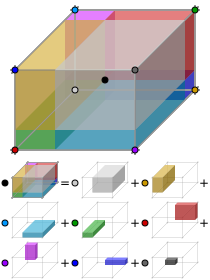
\includegraphics[width=0.5\textwidth]{trilinear.png}
					\caption{Visualization of trilinear interpolation as a~composition of linear interpolations. \textcolor{red}{Image drawn in GeoGebra and inspired by \href{https://commons.wikimedia.org/wiki/File:3D_interpolation2.svg}{a~similar image on Wikipedia} (which looks a~bit worse) -- is credit necessary?}}
					\label{fig:trilin}
				\end{figure}
					
				We can also write
					\begin{eqnarray}
						\widehat{f}(\mathbf{C}) = \sum_{i,j,k \in \{0,1\}} t_x^i t_y^j t_z^k f(\mathbf{C}_{ijk}),\\
						t_\alpha \stackrel{\text{def}}{=} \begin{pmatrix}t_\alpha^0\\ t_\alpha^1\end{pmatrix} = \begin{pmatrix}1-\alpha_d\\ \alpha_d\end{pmatrix},
					\end{eqnarray}
				where $\alpha \in \{x,y,z\}$ is an index. This gives a~nice geometric interpretation to the trilinear interpolation as shown in Figure~\ref{fig:trilin2}. Furthermore, we can write $\widehat{f}(\mathbf{C})$ as a~polynomial:
					\begin{equation}
						\label{eq:trilinpoly}
						\widehat{f}(\mathbf{C}) = \sum_{\alpha,\beta,\gamma \in \{0,1\}}\sum^{\alpha}_{i=0}\sum^{\beta}_{j=0}\sum^{\gamma}_{k=0} 	(-1)^{(\alpha-i)+(\beta-j)+(\gamma-k)} f(\mathbf{C}_{ijk}) x_d^\alpha y_d^\beta z_d^\gamma.
					\end{equation}
				We take advantage of this form when generalizing trilinear interpolation to irregular grid in section~\ref{sec:interpol}.
					%\begin{equation}
					%	\widehat{f}(C) = (1-x_d) (1-y_d) (1-z_d) f(C_{000}) + (1-x_d) (1-y_d) z_d f(C_{001}) + (1-x_d) y_d (1-z_d) f(C_{010}) + (1-x_d) y_d z_d f(C_{011}) + x_d (1-y_d) (1-z_d) f(C_{100}) + x_d (1-y_d) z_d f(C_{101}) + x_d y_d (1-z_d) f(C_{110}) + x_d y_d z_d f(C_{111})
					%\end{equation}
					
				\begin{figure}
					\centering
					\includegraphics[width=\textwidth]{trilinear2.png}
					\caption{Geometric interpretation of trilinear interpolation. The~colored dots represent the~values in given points and the~colored boxes represent the volume by which the~corresponding values are multiplied. The~black dot represents the~interpolated value which is multiplied by the entire volume~\cite{trilinear}.}
					\label{fig:trilin2}
				\end{figure}
				
				\textcolor{red}{Maybe a~citation here, although I am not sure it is necessary since it could be considered common knowledge. The~last two equations are my own. Maybe $x_0$, etc. should be explicitly described.}